\chapter{Introduction}
\label{cha:intro}

The mobile industry is without a doubt one of the most vibrant industries at the moment. It is characterized by rapid growth and intense competition which has led to fragmentation. This chapter first presents an overview of the evolution in the mobile device landscape, then explains the problem of fragmentation and how cross-platform tools (CPTs) can help solve this problem and finally, the goals of this thesis are defined.

\section{The mobile device landscape}

In this first section, the mobile device landscape and its evolution will be explored. It will introduce the concepts of smartphones, tablets and mobile operating systems and illustrate their popularity using worldwide sales numbers.

\subsection{Smartphones}

Mobile phones have been around for a while now but ever since the (nearly simultaneous) introduction of the iPhone 3G and the HTC Dream in 2008, smartphones are taking over from traditional cell phones or feature phones. A feature phone (sometimes also called a dumb phone) is a low-end mobile phone, providing only basic telephony and texting. Smartphones on the other hand are high-end devices that combine the functionality of mobile phones with the functionality of a portable computer. These devices have advanced computing power and often include multiple connectivity options (cellular, Wi-Fi, Bluetooth, NFC, etc.), sensors (GPS, compass, accelerometer, etc.), applications, etc. In the last five years, smartphone sales have grown tremendously. According to quarterly studies by Gartner\footnote{Gartner is an American research and advisory firm, specialized in information technology, \url{http://www.gartner.com}.} \citeGartner, smartphone sales have grown 544\% since the second quarter of 2008 (see \fref{fig:smartphone-sales}). Smartphones are becoming ubiquitous and in some regions like the United States, smartphone penetration (this is the ratio between smartphones and all mobile phones) has already reached more than 50\% \cite{Nielsen:2012}. 

\begin{figure}[h]
    \begin{center}
        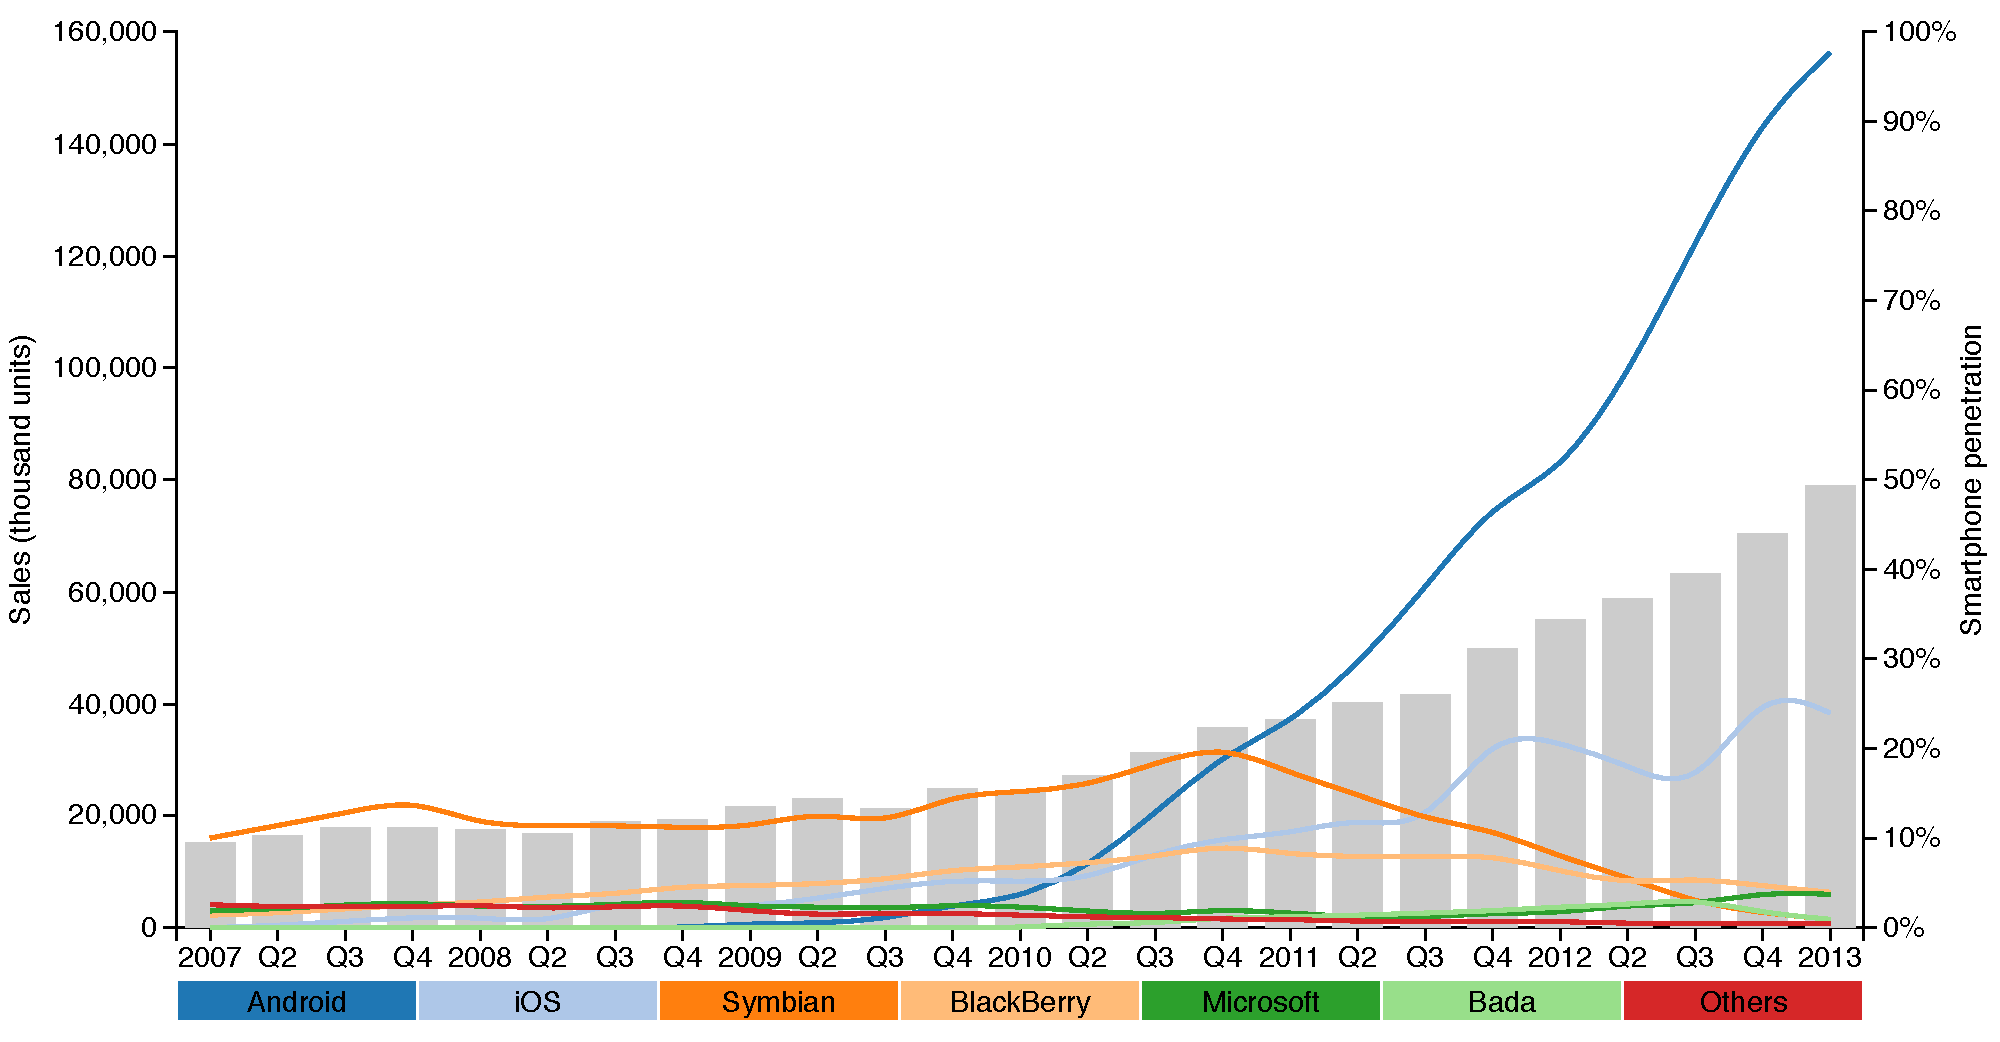
\includegraphics[width=\textwidth]{figs/smartphone_sales.pdf}
        	\caption{
        	    Evolution of worldwide smartphone sales by operating system (lines) and smartphone penetration (bars). Source: Gartner \citeGartner
        	}
        	\label{fig:smartphone-sales}
    \end{center}
\end{figure}

Each of these smartphones comes with a mobile operating system which allows owners to run third-party software, typically called apps, on their device. These operating systems or platforms, are heavily subjected to network effects, i.e. their value is dependent on the number of people using it. This makes it hard for new platforms to gain traction which is visible in \fref{fig:smartphone-sales} and \fref{fig:smartphone-share}. Android and iOS are currently dominant and other platforms are either in decline (like Symbian and Blackberry, formerly RIM) or have a hard time getting traction (like Windows Phone, the successor of Windows Mobile, which already existed before Android and iOS).

\begin{figure}[h]
    \begin{center}
        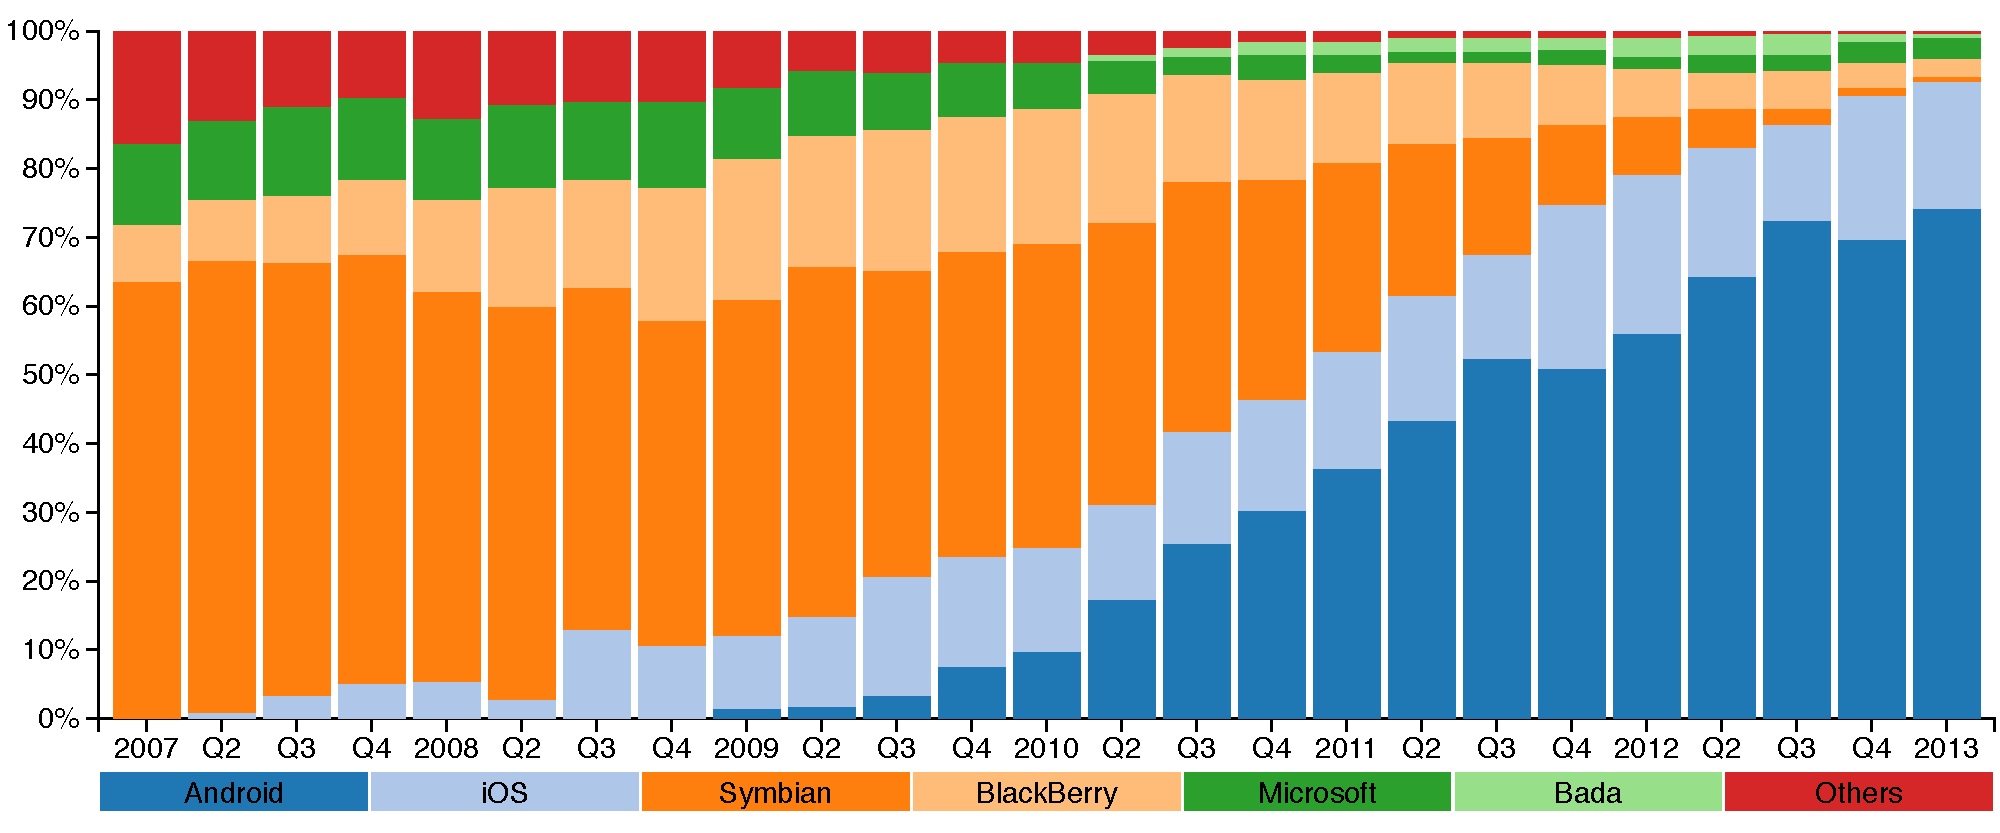
\includegraphics[width=\textwidth]{figs/smartphone_share.pdf}
        \caption{
            Evolution of worldwide smartphone market share by operating system.\newline 
            Source: Gartner \citeGartner
        	}
        \label{fig:smartphone-share}
    \end{center}
\end{figure}

However, there is no single major platform. In addition, the IDC\footnote{International Data Corporation is another American research, analysis and advisory firm, specializing in information technology, telecommunications and consumer technology, \url{http://www.idc.com}.} predicts that Windows Phone will gain a significant market share by 2016 and that 90\% of the worldwide smartphone market will then be covered by Android, iOS and Windows Phone \cite{IDC:phone}. Hence, it is reasonable to assume that there will always be more than one major platform.

\subsection{Tablets}

The second type of mobile devices are tablet computers or tablets. In their current form, tablets are somewhat similar to smartphones but they have larger touchscreens (customarily starting at 7 inches in diagonal) and do not offer basic telephony. However, some of them do have a cellular radio that can be used for data transmission. Because of their hardware similarities, their software is also similar: the dominant smartphone operating systems are also used in tablets.

As with smartphones, tablets gained a lot of popularity since the launch of the iPad and Android tablets. According to other studies by both Gartner \citep{Gartner:11tab,Gartner:12tab} and the IDC \citep{IDC:tablet}, tablets will continue to gain popularity and sales will be mainly driven by iPads and Android tablets (see \fref{fig:tablet}). Even though these studies disagree on which operating system will be used in most devices, they both predict there will be three major platforms: iOS, Android and Windows. 

\begin{figure}[h!]
    \begin{center}
        \TODO{Merge graphs into one image, this is UGLY!}
        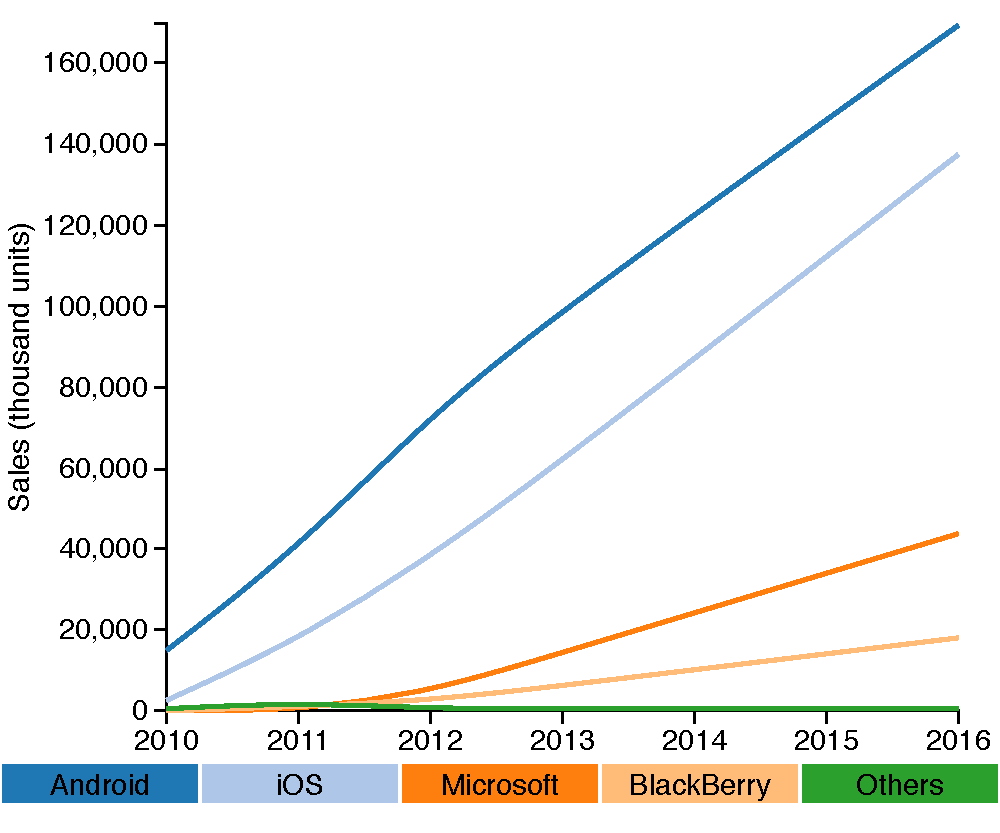
\includegraphics[width=0.49\textwidth]{figs/tablet_sales.pdf}
        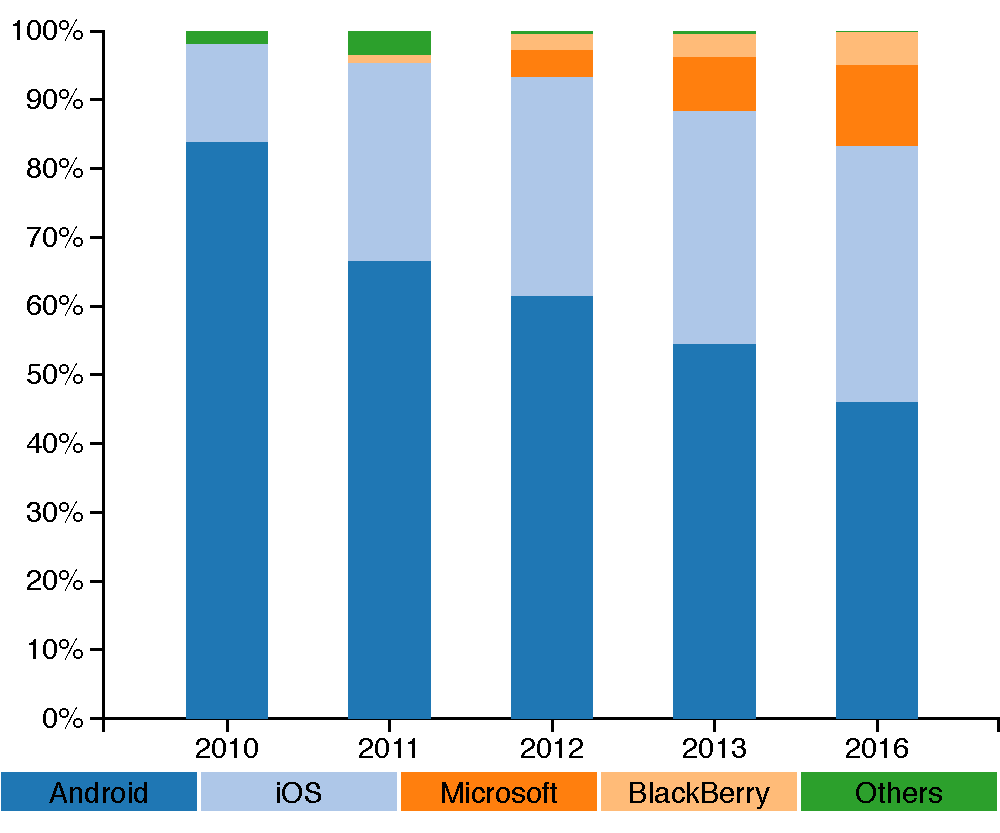
\includegraphics[width=0.49\textwidth]{figs/tablet_share.pdf}
        \caption{Prediction of worldwide tablet sales and market share.\newline Source: Gartner \citeGartnerTab
        }
        \label{fig:tablet}
    \end{center}
\end{figure}

\section{The problem of fragmentation}

This section focusses on the problem of fragmentation. Fragmentation can be defined as the fact that all devices are different; there is no uniform device. This is called device fragmentation. In fact, all mobile devices can be divided into multiple, overlapping categories like operating system or platform (called platform fragmentation), operating system version or runtime (called runtime fragmentation), screen size and screen resolution (called screen fragmentation) and many more. Hence, fragmentation is a multi-dimensional platform. 

Fragmentation is generally beneficial for consumers, carriers and manufacturers. The more different devices there are, the more likely a consumer will find a device that fits his needs. For developers on the other hand, fragmentation is usually disadvantageous. It forces them to test their applications on multiple devices to guarantee the desired user experience. This is expensive and time-consuming. 

The nature of a platform strongly influences the fragmentation issues within said platform. For instance, Apple can manage fragmentation issues pretty well because iOS is a closed platform and the only devices running iOS, called iDevices, are designed by Apple itself. In fact, these devices show many similarities. Android on the other hand is an open system. Android is being developed privately at Google, but the source code of every release is publicly available under the Apache 2.0 License, which means that everybody is allowed to customize it. The ability for manufacturers to alter the operating system has largely contributed to the success of Android. \TODO{Update: On April 24 2013}, the Google Play Store\footnote{Google Play is the official marketplace for Android applications.} listed 2827 officially supported device configurations, distributed across 59 manufacturers. 

Mobile device manufacturers are eager to modify the Android operating system to differentiate their product from their competitors. As such, they create their own Android flavour, i.e. a distribution of Android with a custom user interface (like HTC Sense, Samsung TouchWiz, etc.), custom software, additional market places, etc. However, reapplying these modifications for every new release of Android is cumbersome and costly which is why device manufacturers do not often provide updates for their devices. This has led to the notorious Android runtime fragmentation, which is depicted in \fref{fig:android_runtimes}. The adoption rate for new versions is low and is caused by the nature of Android. Developers have to support multiple versions, which is tedious. 

\begin{figure}[h]
    \begin{center}
        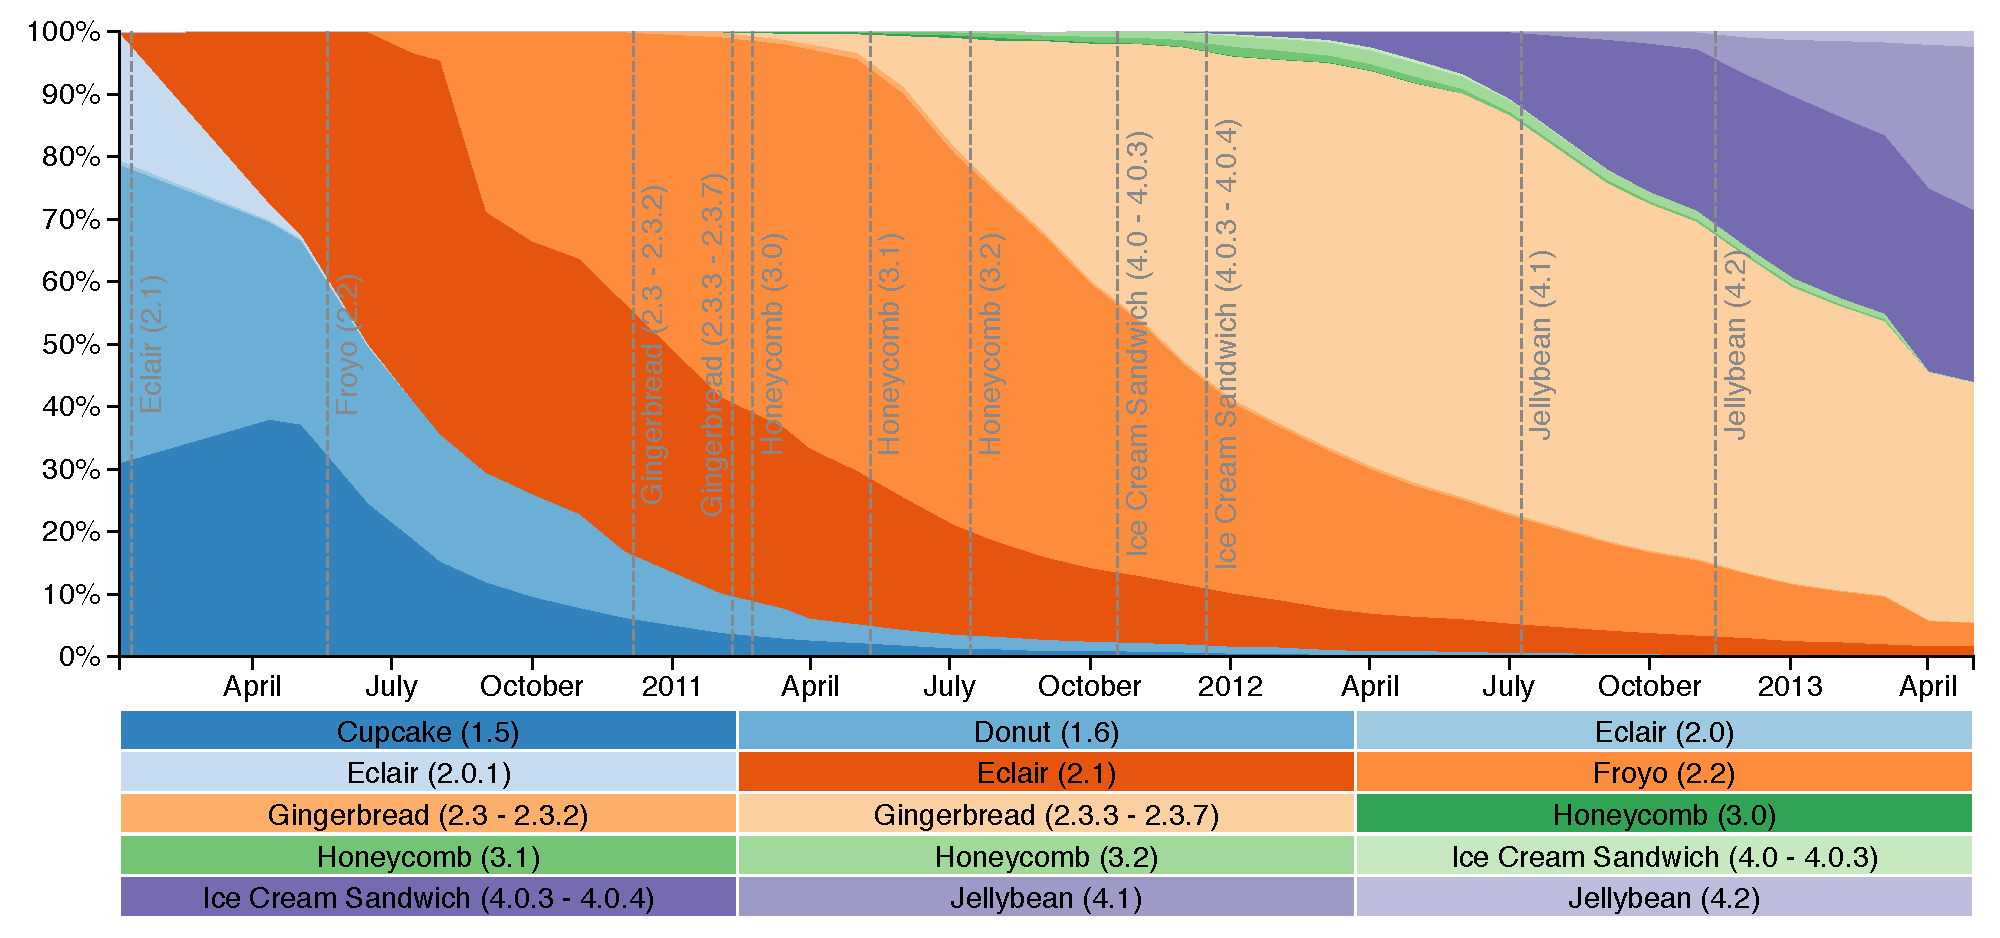
\includegraphics[width=\textwidth]{figs/android_runtimes.pdf}
        \caption{Historical Android runtime fragmentation. The data for this graph was aggregated from \cite{Android:Versions} using the Internet Archive (\url{http://archive.org}).}
        \label{fig:android_runtimes}
    \end{center}
\end{figure}

Unlike Google, Apple does not publicize runtime statistics but developers \cite{Smith:2013} and online advertisers \cite{Chitika:2013} can confirm fast adoption rates for iOS. On iOS, developers can make use of new functionality much faster. However, some devices that are still being used (like the original iPad and the iPod third generation) did not receive an update to iOS 6. Because of this, iOS developers now have to support the two latest versions of iOS.

Android and iOS are used in both smartphone and tablets. The number of different screen sizes and resolutions is low on iDevices. In contrast, there is an enormous number of screen sizes and resolutions on Android devices. This implies that applications also have to deal with various screen sizes and resolutions. On Android, this is solved by a flexible layout system. On iOS, this is solved by centering the user interface in the middle of the screen. For instance, applications that are not optimized for the 4-inch display of the iPhone 5 (or iPod Touch, 5th generation) will have black bars on the top and the bottom. Retina displays do not really introduce a new screen resolution because every logical pixel is represented by four physical pixels and this conversion is mostly handled by the operating system.

There are still a lot more dimensions to the fragmentation problem like computing power, available sensors, available networking, etc. but these differences can be categorized under device fragmentation. In concluding, fragmentation among Android devices is rather high, fragmentation among iDevices is rather low.

\section{Cross-platform tools to the rescue}

In the current economy, information is a company's most valuable asset and the rate at which information exchange takes place increases every day. Mobile Internet-enabled devices are a valuable resource for this purpose and, as a consequence, many companies want mobile applications for their businesses. However, in an ever-changing and unpredictable industry like the mobile industry, it is unwise to target a single platform. This could eventually lead to vendor lock-in, i.e. all operations (or a significant part thereof) depend on equipment or software of a single vendor and switching vendors would require high costs. Companies will try to avoid  these situations at all costs and they will do so by asking for cross-platform solutions. 

These cross-platform solutions typically require that the software is implemented multiple times, one time for each platform. This is costly and time-consuming. Cross-Platform Tools (CPTs) can help to solve this problem because they allow to support multiple platforms from a single codebase. Hence, they lower entry barriers (access to new platforms) and exit barriers (lock-in) \cite{VMCPT:2012}. 

Cross-Platform Tools try to solve three major problems \cite{VMCPT:2012}: 

\begin{enumerate}
    \item \textbf{Fragmentation} Fragmentation issues as described above are a struggle for every developer. They are forced to test their applications on a large number of devices in order to be able to guarantee the desired user experience. A CPT can help to identify platform quirks and provide workarounds. 
    \item \textbf{Access to new platforms} Targeting a new platform is generally hard. Developers have to learn yet another SDK and/or programming language in order to deliver applications for this platform. A CPT can make abstraction of platform differences which allows developers to reuse their current skills. This drastically reduces the effort that is needed to target a new platform. Note that a new platform does not necessarily have to be a smartphone or tablet operating system, it could also be the operating system of a television set or a car console, etc.
    \item \textbf{Development inefficiency} Maintaining codebases for multiple platforms is a difficult and costly task. When a new feature is introduces, it has to be applied to all codebases. With the use of a CPT, all code is contained within a single codebase and no time is lost while synchronizing features and other maintenance tasks across codebases. This reduces cost and increases productivity. 
\end{enumerate}

\section{Goals}

This last section defines the goals of this thesis. From the introduction, it is clear that there is a large demand for cross-platform solutions and that there are a lot of benefits associated with the use of cross-platform tools. Therefore, this thesis will try to identify a suitable cross-platform tool for mobile application development. This is a two-step process. First, a methodology will be defined for evaluating and selecting cross-platform tools. Second, this methodology will be used to evaluate a number of alternatives and to select the best-suited alternative.